%% LyX 1.5.0 created this file.  For more info, see http://www.lyx.org/.
%% Do not edit unless you really know what you are doing.
\documentclass[11pt,english]{article}
\usepackage[T1]{fontenc}
\usepackage[latin9]{inputenc}
\usepackage{geometry}
\geometry{verbose,letterpaper,tmargin=1in,bmargin=1in,lmargin=1in,rmargin=1in}
\usepackage{graphicx}

\makeatletter

%%%%%%%%%%%%%%%%%%%%%%%%%%%%%% LyX specific LaTeX commands.
%% Because html converters don't know tabularnewline
\providecommand{\tabularnewline}{\\}
%% A simple dot to overcome graphicx limitations
\newcommand{\lyxdot}{.}


\usepackage{babel}
\makeatother

\begin{document}

\title{Getting started with Aruspix.}

\maketitle

\section{Introduction}

Aruspix is a program for the application of optical recognition to
early printed music sources. Starting with scanned images of these
early sources, Aruspix will first pre-process the image, to clean,
correct and pre-classify the various elements, then digitally recognize
the image for musical content. This two-step process can be applied
to single pages, or to an entire book, or batch, of pages. When working
with books, an optimization process can be applied after a significant
number of pages (approx. 20) has been corrected. The optimization
process will improve results for the recognition of the book. Your
prepared images for use with Aruspix must be stored as TIFF files.
A resolution of at least 300 dpi is recommended. Each single file
or image should contain only one page of music.

To begin using Aruspix, have a look at the two menus at the top of
the screen. The upper menu is like the one for most applications \textendash{}
File, Edit, Window, etc. This will be called the Application menu
(Figure \ref{fig:Menu-bar}). Directly below the Application menu
bar, you will see another menu bar with helpful graphics \textendash{}
New \& Open for a book, New and Open for a file, Save, etc. This will
be called the tools bar (Figure \ref{fig:Tool-bar}). 

%
\begin{figure}[h]
\begin{centering}

\includegraphics[scale=0.5]{ApplicationMenu}
\par\end{centering}

\caption{Menu bar\label{fig:Menu-bar}}



\end{figure}


%
\begin{figure}[h]
\begin{centering}
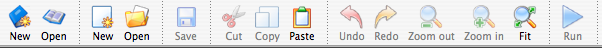
\includegraphics[scale=0.5]{ToolBar}
\par\end{centering}

\caption{Tool bar\label{fig:Tool-bar}}



\end{figure}



\section{Processing a single page}

The first thing you need to do to start transcription is to pre-process
the music images you wish to transcribe. For now, we will begin with
a single page. From the tool bar, click on the third icon 
\includegraphics[height=1em]{OpenNewFileButton}.
Find the file {}``MarL\_1585\_M.0578\_I.Nc.2\_01\_028'', and double-click
on it to open it. You should now see the image that you are going
to work with as in figure \ref{fig:Image-processed}. If at any time
the image you are working with does not fit the screen, use the {}``Zoom''
buttons on the tool bar 
\includegraphics[height=1em]{ZoomButtons}
to adjust the image size.

%
\begin{figure}[h]
\begin{centering}
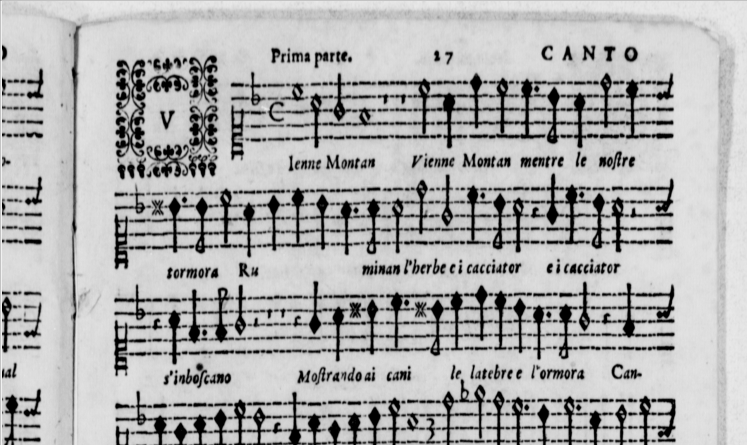
\includegraphics[scale=0.5]{ScannedTextRaw}
\par\end{centering}

\caption{Image to be process\label{fig:Image-processed}}



\end{figure}


To pre-process this image, click {}``Run'' on the tool menu 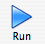
\includegraphics[height=1em]{RunButton}.
In a few seconds the pre-processed version of this page will appear
on your screen. Once your page is pre-processed, the first editing
step must be done. The page is color coded during pre-processing,
and it is necessary to check that everything is correctly labeled.
In this example, there is only one correction to be made: there is
a bit of black border on the upper left-hand side of the image which
should be erased. Double-click on any part of the black border, and
it will all turn red (Figure \ref{fig:Correction-preprocessing}).
To erase the border, right-click (or <ctrl-click>) over the red, and
a colour-menu will appear (Figure \ref{fig:Pre-processing-categories}).
Choose {}``blank'', and the border will fade out.

%
\begin{figure}[h]
\begin{centering}
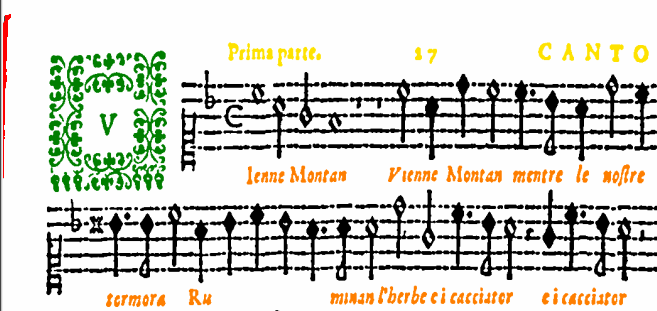
\includegraphics[scale=0.5]{BlackBorderRed}
\par\end{centering}

\caption{Correction of the pre-processing\label{fig:Correction-preprocessing}}



\end{figure}


%
\begin{figure}[h]
\begin{centering}
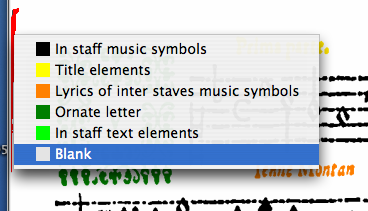
\includegraphics[scale=0.5]{PPCorrection}
\par\end{centering}

\caption{Pre-processing categories\label{fig:Pre-processing-categories}}



\end{figure}


Once the page has been corrected at this stage, it is ready for transcription.
Simply click on the \textquotedblleft{}Run\textquotedblright{} icon
for a second time, and wait a few seconds for the process to complete.
If the dialogue box with the transcribing process information seems
to stop and become idle, make sure the command \textquotedblleft{}Close
this dialog if process completes successfully\textquotedblright{}
is selected with a tick. This will ensure that in future you will
not have to close the dialogue box yourself every time you transcribe
a page. What should appear before you is a screen split into two sections,
with your original page showing on the top half, and the newly transcribed
page lined up below (Figure \ref{fig:Page-after-recognition}). In
between the two screens is a third menu bar, the music editing bar.

%
\begin{figure}[h]
\begin{centering}
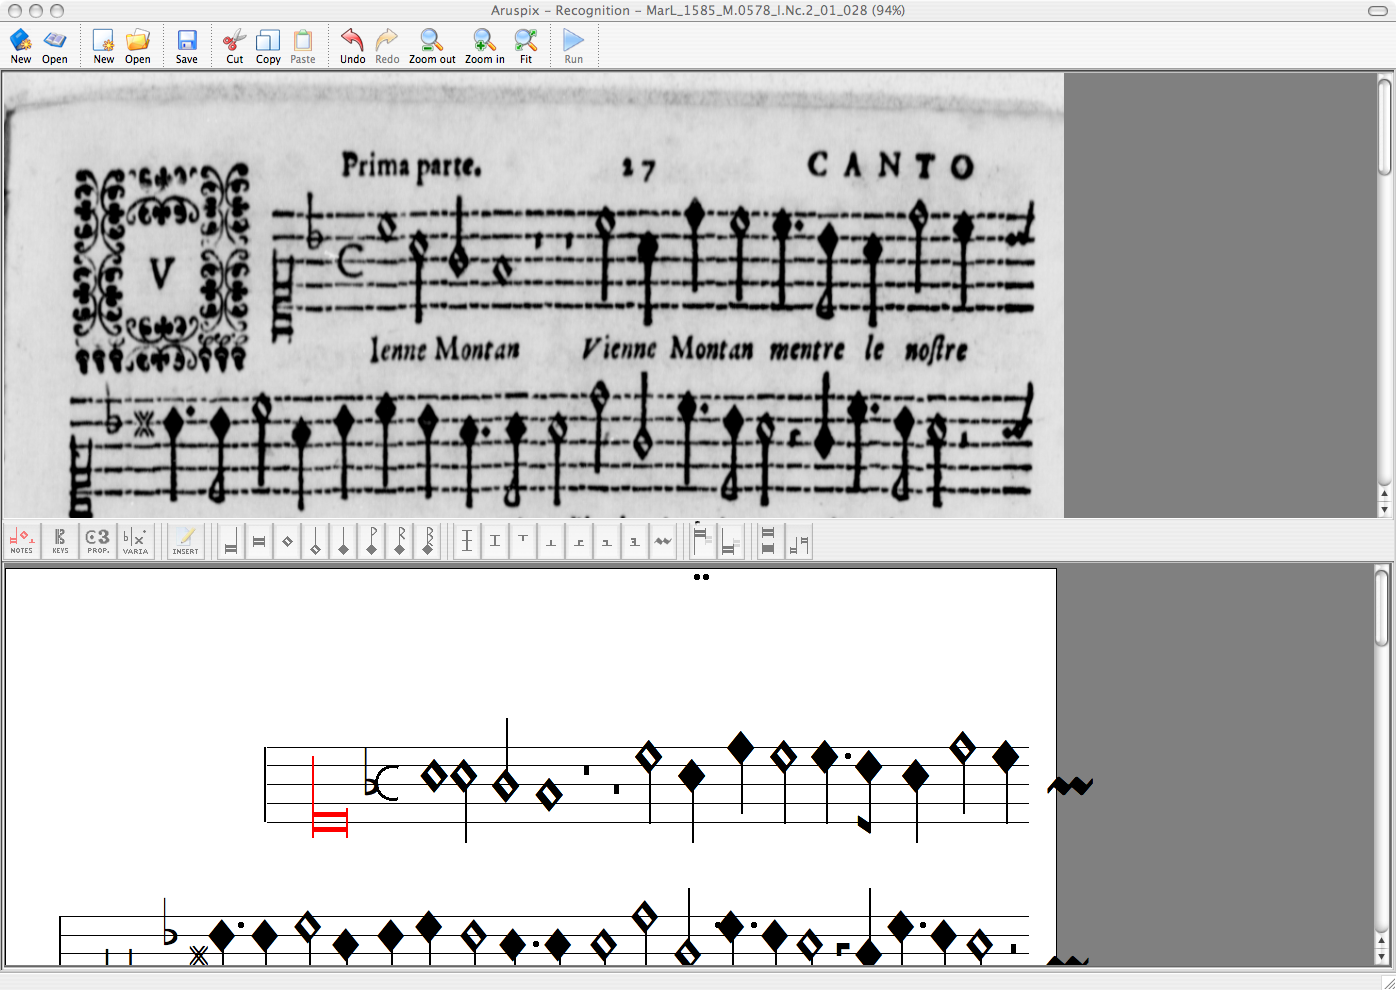
\includegraphics[scale=0.25]{EditScreen}
\par\end{centering}

\caption{Page after recognition\label{fig:Page-after-recognition}}



\end{figure}


Before you begin making corrections, it is a good idea to learn how
to move around the page and familiarize yourself with the interface.
For now, you will be working on the bottom screen - the top screen
will be for reference only. As you can see, the first symbol on the
bottom screen is red, while the rest are black. The red symbol indicates
where Aruspix is focussed - it is the cursor. Click on any symbol,
and it will become red. You can also use the arrow keys to move around
the page. There can only be one red symbol at a time - you cannot
work with multiple symbols.

While you move around the score, you may notice that the music editing
bar changes from time to time. Musical symbols in Aruspix are grouped
into families, and the entire family of each symbol will appear in
the editing bar when one of its members is highlighted. If you return
the cursor to the top of the page, you will see that the first symbol
is a long, and the Notes family shows in the editing bar. Move the
cursor to the next symbol, the flat, and the editing bar will now
show the variants family. 

Any member of a family of symbols is interchangeable with any other
member of the same family. If you go back the first symbol again,
and then click on the Semi-Minim 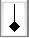
\includegraphics[height=1em]{SemiMinim}
in the editing bar, the Long will be changed into a Semi-Minim. Try
changing it back by clicking on the Long button in the editing bar.

As you can see by comparing the two screens, the first long should
actually be a clef. Because notes and clefs are in different families,
you cannot transform the Long into a clef. You must delete it and
then replace it. To delete the Long, click on it and then press <delete>.
You can use either of the two delete keys (see reference for more
details). Once the Long has been deleted, click on {}``Insert''
in the editing bar 
\includegraphics[height=1em]{InsertButton}. The
arrow for the mouse should become a pencil. Next, use the pencil to
click on the {}``Keys'' button and select the third clef 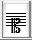
\includegraphics[height=1em]{CantoClef}.
Double-click on the staff where you want to insert this clef, and
it will appear. To return to the editing mode, select {}``Edit''
from the editing bar 
\includegraphics[height=1em]{EditButton}, and
the pencil will be replaced by the arrow. You will need to click on
a symbol to make the cursor reappear.

The next correction that needs to be made is for the key signature.
The flat is a third too low, and needs to be moved up. There are two
ways to do this, both of which are quite simple. You can either drag
the flat into the right place using the mouse, or select it and use
<ctrl-arrow up> or <ctrl - arrow down> to move it up or down one pitch
at a time. Try moving the flat up and down using these two methods.

There are three more corrections for the first line that are exactly
the same as for the key signature. The first note, the second rest,
and the custos are all a third too low, and need to be moved up. The
seventh note, a Minim, needs to be changed into a Semi-Minim. You
can do this the same way you changed the initial Long into a Semi-Minim:
Click on the Minim, then click on the Semi-Minim in the editing bar.

Once you have done this, use the right arrow key to move the cursor
to the second line and continue editing. The sharp in front of the
first note needs to be moved up, and also the custos. Move on to the
third line - first rest needs to be changed from a minim rest to a
semi-minim rest. Then the third rest of the next group of rests needs
to be moved down. The breve before the next fusa (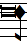
\includegraphics[height=1em]{FusaWithBreve})
needs to be replaced with a sharp. Delete the breve, and then try
a short-cut for inputting the sharp. Make the sure fusa is selected
and then press <d>. The sharp should appear at the correct pitch.
There is a similar shortcut for inputting flats - press <b>. There
is no shortcut for the natural sign.

As you continue to practice editing this page, you should find that
simple replacements, deletions, or pitch corrections are the only
procedures you need to use. At the end of the piece, you will need
to delte the extra long and clef, and then insert two single bar lines
to create the final double bar line. The bar line is found in the
variant family, second to last 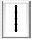
\includegraphics[height=1em]{BarLine}.
Do not confuse this with the Long rest, found in the notes family
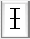
\includegraphics[height=1em]{LongRest}. Erase the extra bar-line
in the final staff, and you are finished making corrections.

The final step in editing is adjusting the alignment - making sure
that the symbols on the bottom screen are aligned with those on the
top screen. This cannot be done just by looking, so there is a special
tool in Aruspix for this procedure. Move the cursor to the first clef
at the top of the page, then press <ctrl-b>. This activates the highlight
function, and you will see on the top screen that a row of hand-drawn
blue symbols appears overtop of the original image (Figure \ref{fig:Highlighted-transcription}). 

%
\begin{figure}[h]
\begin{centering}
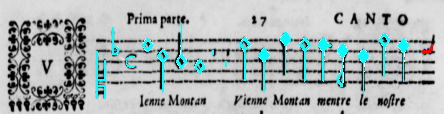
\includegraphics[scale=0.5]{Highlight}
\par\end{centering}

\caption{Highlighted transcription in the original image\label{fig:Highlighted-transcription}}



\end{figure}


The cursor now appears in both screens simultaneously. To move any
of the blue symbols on the top screen, you need to move the corresponding
symbol on the bottom screen. Try to align the blue symbols with their
matching symbols underneath as closely as possible, either by dragging
them with the mouse, or by using the following keyboard commands:

\begin{itemize}
\item move to the right: <space bar>
\item move to the left: <ctrl - spacebar>
\item move up: <ctrl - up arrow>
\item move down: <ctrl down arrow>
\end{itemize}
When the page is aligned, click {}``Save'' to store the corrections.


\section{Processing a whole book.}

Aruspix can also deal with whole books or compilations of pages, providing
a visual index for the book while you work on individual pages within
it. It is much more convenient to pre-process an entire book all at
once than to run each page separately. In order to do this, you need
to make a file for the book or compilation of pages, and prepare a
place to store these pages once they have been edited with Aruspix.
As before, each page within your book should only contain a single
page of music, and be stored as a TIFF file.

Open Aruspix, and click on the {}``New book'' icon in the tools
bar 
\includegraphics[height=1em]{NewBookIcon}. A window will open
with several meta-data fields that you can use to label your book
(Figure \ref{fig:Book-metadata}). 

%
\begin{figure}[h]
\begin{centering}
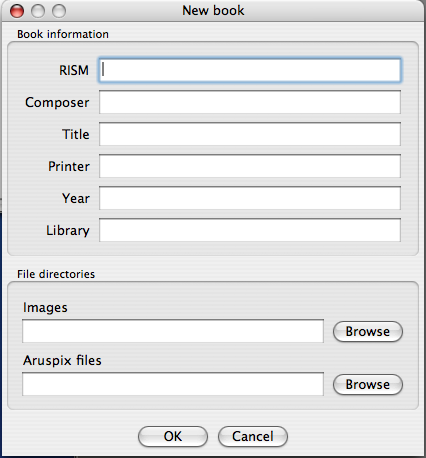
\includegraphics[scale=0.5]{NewBookWindow}
\par\end{centering}

\caption{Book metadata\label{fig:Book-metadata}}



\end{figure}


All of these fields are optional. If you have a particular name that
want to use for your book, instead of the suggested fields, type that
name into the RISM field. For now, we will use a demo book, and fill
in all the optional fields:

\begin{itemize}
\item The RISM number is M.0578.
\item The Composer is Luca Marenzio.
\item The Title of the Book is {}``Libro Primo. Madrigali a 4 voci''
\item The printer is Alessandro Gardano.
\item The Year of printing is 1585.
\item The Library code is I.Nc.2
\end{itemize}
Once you have labeled your book, you need to indicate where the images
are stored on your computer, by browsing through the locations under
the heading {}``Images''. {[}find out where these files will be
located if they come as part of the Aruspic demo]. Below that, you
need to indicate where the edited images should be stored once they
are saved in Aruspix. You may choose to store the demo files on your
desktop for now, or create a folder for them somewhere else. When
you have filled in all the fields for this window, click OK.

You will see that the Aruspix screen is now divided into two sections.
You have your book directory on the left, and a working space on the
right. Before you can pre-process the book, you need to ensure that
only pages that contain music will be run. If you open the file that
is labeled page 01\_001.tif. you will see that it is a blank page.
Right click on the file, and you can choose {}``deactivate'' from
the menu that appears (Figure \ref{fig:Images-desactivated}). This
will make the file name turn grey. Do this to the following page as
well, since it is a title page and contains no music.The following
pages from this book need to be deactivated: 

\begin{itemize}
\item Part 01 pages 31-32. 
\item Part 03 pages 1-3.
\item Part 04 pages 1-3.
\end{itemize}
%
\begin{figure}[h]
\begin{centering}
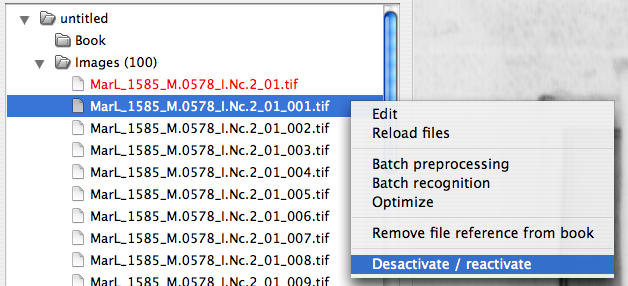
\includegraphics[scale=0.5]{FileDeactivation}
\par\end{centering}

\caption{Images in a book can be desactivated or reactivated\label{fig:Images-desactivated}}



\end{figure}


{[}there is an existing aruspix file that needs to be removed for
the demo, as well as some red pages that should not appear here.]
Once all the non-music files are deactivated, you can pre-process
the entire book by clicking {}``Book'' in the application menu and
choosing {}``Batch preprocessing'', or by right-clicking on any
file in the book and choosing {}``Batch preprocessing'' from the
menu that appears. Preprocessing will take approximately 1 minute
per page.

After the preprocessing has finished, you should find a new directory
of pages in the Aruspix files folder, just below the Images folder
on the left-side of the screen. These are the files that you will
be using from now on.

If you open the first page in the Arupsix files, 01\_003, you will
see the colour-coded version of the page that Aruspix will be working
with.

From here, you can follow the same steps that you used in the demo
for processing a single page.

There are no corrections in the preprocessing for this page.

Click {}``Run'' in the tools menu, and wait for recognition to complete.
(About 10s)

Now you are in the editing mode, and the Arupsix window is divided
into three parts. As with the single page, you would at this point
edit the page and correct the alignment, using the editing tools and
keyboard shortcuts. For this demo, it is not necessary to edit the
page. Simply click on the {}``Save'' icon, which will make a green
tick appear beside the file on the left screen. Ordinarily it is suggested
that you edit about twenty pages, making all the necessary corrections,
before you optimize the results. Running a full optimization will
improve Aruspix's recognition for the specific book that you are editing,
so it is worthwhile to do this once you have enough pages completed.
Simply choose Book from the Application menu, and then Optimize.

The time needed for this process depends on the number of pages you
use. Twenty pages takes about 50 minutes, while ten pages takes only
about 20 minutes. Optimization is always a cumulative process, so
if you run a full optimization every twenty pages, the second time
will take about an hour and 45 minutes, since there will be 40 pages
included in the run.

There are a number of editing tasks and tools that have not yet been
discussed, but which will be worth reading about before you proceed
with your first editing project. These can be found in the Editing
Reference section.


\section{Editing Reference}


\subsection{Explanation }

\begin{itemize}
\item Aruspix acts at the graphic level, which means that every element
is independent. For example, a dotted note with a flat is represented
by 3 elements (a flat, a note, and a dot) and each element is edited
separately. Merging is performed during exportation. Similarly, when
a clef is modified, elements are internally transposed to keep the
same graphical representation \textendash{} there will be no visual
indication in the editing mode that anything has been transposed.
Other examples of symbols composed of more than one element are the
F clef, the ligatures, key signatures and some time signatures. For
key signatures that use the octave flats or sharps, the two symbols
combined will be treated, exceptionally, as a single symbol, and represented
by the lower element for functions such as insertion, editing and
alignment. 
\item Aruspix differentiates between pitched elements (notes, rests, accidentals,
etc.) and unpitched elements (barlines, clefs, time signatures, etc.)
Only pitched elements can be moved up or down. 
\item There is a simple distinction between the editing mode and insertion
mode: in the editing mode, symbols may be moved, converted, or deleted.
In the insertion mode, the only operation that may be performed is
insertion.
\end{itemize}
%
\begin{figure}[h]
\begin{centering}
\begin{tabular}{ccc}
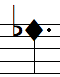
\includegraphics[scale=0.5]{DottedNoteWithFlat} & 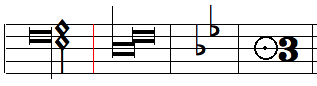
\includegraphics[scale=0.5]{SpecialSymbols} & 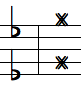
\includegraphics[scale=0.5]{OctaveKeySignatures}\tabularnewline
\end{tabular}
\par\end{centering}

\caption{Examples of symbols}

\end{figure}



\subsection{There are two universal editing functions for all symbols: }

Insertion or deletion. 

Horizontal adjustment/alignment.


\subsection{There is an additional specific editing function for pitched elements: }

Vertical adjustment \textendash{} change of pitch.


\subsection{Editing functions for notes/rests:}


\subsubsection{Change duration:}

There are several ways to do this. You can select the note/rest that
needs to be changed, and then click on the desired note/rest in the
editing bar to make the change. You can select the note/rest that
needs to be changed and then enter the corresponding number (0-7)
of the desired note, or <ctrl + 0-7> for the desired rest. You can
select the note that needs to be changed, and use <ctrl + left or
right arrow> to increase or decrease the duration. This function is
not applicable to rests.


\subsubsection{Change pitch}

There are two ways to change the pitch of a notee/rest. Either drag
the symbol with the mouse, or select the symbol and use <ctrl \textendash{}
up or down arrow> to adjust the pitch.


\subsubsection{Add an accidental to a note}

There are two ways to add accidentals to a note: You can insert any
accidental using the mouse, by going into the Insert mode and selecting
the desired accidental from the variant family, then inserting the
accidental where you want it in the staff. They can be adjusted using
<ctrl \textendash{} up or down arrow>, <space bar> or <ctrl \textendash{}
space bar>. You can use a keyboard shortcut to insert a flat or a
sharp. Select the note to which the accidental should apply, then
press <d> for a sharp or <b> for a flat. The accidental will appear
before the note, and at the correct pitch. There is no keyboard shortcut
for the natural sign.


\subsubsection{Add a dot to a note}

There are two ways to add a dot to a note: Using the mouse, you can
enter the Insert mode, select the dot from the variant family, and
double-click on the staff where you want the dot to appear. Dots can
be moved in any direction using <ctrl \textendash{} up or down arrow>,
<space bar> or <ctrl \textendash{} space bar> . You can also add a
dot by selecting the note to which it should be applied, and pressing
< . > The dot will appear at the correct pitch after the note.


\subsubsection{Change the stem orientation}

There are two ways to change the orientation of the stem: You can
select the note and then click on the last button in the notes family.
(Graphic) You can also select the note and press < a >. 


\subsubsection{Change the coloration}

There are two ways to change the coloration of a note: You can select
the note and click on the next-to-last button in the notes family.
(Graphic) You can also select the note and press < i >.


\subsubsection{Ligatures }

There are two ligature formations available in the notes family menu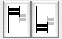
\includegraphics[height=1em]{LigatureButtons}.
Because Aruspix functions at the graphic level, it is necessary to
combine two or more separate symbols to create a ligature while you
are editing a page. When the page in later exported, the separate
symbols will be fused into one symbol. To create a ligature, enter
the Input mode and use the mouse to select one of the two ligature
symbols. Insert it onto the staff by double-clicking, and then add
a breve in the same way. There will be new ligatures coming soon.
. . (2 more coming)

%
\begin{figure}[h]
\begin{centering}
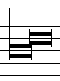
\includegraphics[scale=0.5]{LigatureSample}
\par\end{centering}

\caption{COP ligature composed of two symbols}



\end{figure}



\subsection{Editing Functions for Clefs }

Clefs can only be inserted using the mouse. To change a clef, there
are two options:

\begin{itemize}
\item You can select the clef, and then click on the correct clef from the
clef family. 
\item You can select the clef, and then use the Function Keys to change
to clef. THIS FUNCTION IS CURRENTLY DISABLED.
\end{itemize}

\subsubsection{F clefs}

To create an F clef in Aruspix, you will need to combine two symbols
\textendash{} a Long and one of the three bass clefs in the clef family
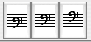
\includegraphics[height=1em]{BassClefButtons} (Figure \ref{fig:F-clefs-symbols}).

%
\begin{figure}[h]
\begin{centering}
\begin{tabular}{cc}
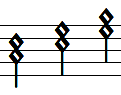
\includegraphics[scale=0.5]{BassClefs} & 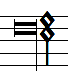
\includegraphics[scale=0.5]{FClef}\tabularnewline
\end{tabular}
\par\end{centering}

\caption{F clefs symbols and a F clef with the additional Long symbol\label{fig:F-clefs-symbols}}

\end{figure}

\subsubsection{Editing Lyrics}

Aruspix also allows users to edit the lyric elements of the music. All lyrics
in Aruspix are associated to a single note and a note may have several lyric
elements associated to it. When an element is selected lyrics or notes that
are associated to it are highlighted in light blue. There are two modes in
Aruspix which allow users to manipulate lyrics. The modes are "Lyric Editing"
mode and "Lyric Insertion" mode. Lyric Editing mode allows users to change
the location of lyrics and their note associations while Lyric Insertion mode
allows users to input new lyrics and modify existing lyrics.
\newline\newline \textbf{Lyric Editing} mode is entered by either selecting an
element with the mouse, or pressing the "T" key. Pressing the "T" key will
select the lyric associated to the currently selected note. 
% \newline NOTE: If the currently selected note has no associated lyrics, a
% new empty lyric element will be created underneath the note, and Aruspix will
%a utomatically go into "Lyric Insertion" mode to allow the user to input the
% new lyric. More on "Lyric Insertion" mode will follow.
\newline In Lyric Editing mode you have the following options:
\begin{itemize}
	\item You can navigate through all the lyrics on a page using the "Up" and
	"Down" arrow keys to move between lyric lines and the "Left" and "Right"
	arrow keys to move between lyrics on a lyric line.
	\item A lyric element can be moved by clicking and dragging it to a new
	location.
	\item A lyric line can be shifted vertically by selecting a lyric element
	on the line and holding down the "CTRL" key and pressing the "Up" or "Down"
	arrow keys.
	\item A lyric's association to a note can be modified by selecting the
	element and holding down the "CTRL" key and then pressing the "Left" or
	"Right" arrow keys. Pressing the "Left" arrow key will associate the lyric
	to the next note on the left and pressing the "Right" arrow key will
	associated it to the next note on the right.
	\item A selected lyric element can be deleted by pressing the "Backspace"
	or "Delete" key.
	\item To exit Lyric Editing mode either press the "T" key or select a
	note using the mouse.
\end{itemize} 
\textbf{Lyric Insertion} mode allows users to insert new lyrics or modify
existing lyrics. There are two ways to enter Lyric Insertion mode. The first is
to select a lyric element that you wish to modify and press the "Return" key.
A bounding box will appear around the lyric and you will now be able to modify
it. The second way to enter Lyric Insertion node is to select a note with no
associated lyric elements and then press the "T" key. This will create a new
lyric element underneath the note.
\newline In Lyric Insertion mode you have the following options:
\begin{itemize}
	\item You can insert and delete characters at the current cursor location
	using the keyboard as you would in any text editor.
	\item You can move the cursor to the left and right using the "Left" and
	"Right" arrow keys. If you move the cursor past the beginning or end of a
	lyric, it will jump to the beginning or end of the next lyric.
	\item With the cursor at the end of a lyric element, you can create a new
	lyric element associated to the next note by pressing the "Space" bar. 
	\item With the cursor at the end of a lyric element, you can create a new
	lyric element separated by a hyphen and associated to the next note by
	pressing the "Tab" key.
	\item Lyric Insertion mode is exited by pressing the "Return" key. This
	will put Aruspix back into Lyric Editing mode.
\end{itemize}    

\end{document}
